\documentclass[12pt,a4paper]{article}
\usepackage[utf8]{inputenc}
\usepackage{geometry}
\geometry{a4paper, margin=1in}
\usepackage{hyperref}
\usepackage{graphicx}
\usepackage{amsmath}
\usepackage{booktabs}
\usepackage{tabularx}
\usepackage{float}
\usepackage{xcolor}
\usepackage{listings}
\usepackage{tikz}
\usetikzlibrary{arrows.meta, positioning, shapes.geometric, fit, calc}

\definecolor{flowblue}{RGB}{224,240,255}
\definecolor{flowgreen}{RGB}{228,246,228}
\definecolor{flowyellow}{RGB}{255,247,214}
\definecolor{flowpurple}{RGB}{239,231,255}
\definecolor{flowred}{RGB}{255,232,232}

\hypersetup{
    colorlinks=true,
    linkcolor=blue,
    filecolor=magenta,
    urlcolor=cyan,
    pdftitle={Phase 1 Architecture Report - DAS 839},
    pdfpagemode=FullScreen,
}

\lstset{
    basicstyle=\ttfamily\small,
    breaklines=true,
    backgroundcolor=\color{gray!10},
    frame=single,
    rulecolor=\color{gray!30},
    keywordstyle=\color{blue},
    stringstyle=\color{red},
    commentstyle=\color{green!60!black}
}

\title{\textbf{Phase 1: Architecture and Design Document}\\DAS 839 -- NoSQL Systems\\End Semester Project}
\author{Multi-Pipeline ETL and Reporting Framework\\for Web Server Log Analytics}
\date{\today}

\begin{document}

\maketitle

\tableofcontents
\newpage

%% ---------------------------------------------------------------
\section{Introduction}
%% ---------------------------------------------------------------
This document presents the proposed architecture, parsing strategy, ETL workflow, batching approach, and relational reporting schema for the DAS 839 End Semester Project. The goal is to design and implement a prototype multi-pipeline ETL and reporting tool that processes NASA HTTP Web Server Logs (Jul 1995: 1,891,714 records; Aug 1995: 1,569,898 records; total $\approx$ 3.46 million records) using four interchangeable processing backends: \textbf{Hive}, \textbf{MapReduce}, \textbf{Pig}, and \textbf{MongoDB}.

For Phase 1, a fully working \textbf{Apache Hive} pipeline is implemented and demonstrated. Apache MapReduce is identified as the second pipeline to be completed before or during Phase 1 if time permits, with Pig and MongoDB scheduled for Phase 2.

%% ---------------------------------------------------------------
\section{Overall System Architecture}
%% ---------------------------------------------------------------
The system is designed as a unified, modular framework with a single controller orchestrating all execution backends. The core principle is \emph{separation of concerns}: the controller, the processing pipeline, the database loader, and the reporting module are independent and interchangeable components.

\subsection{Components}
\begin{itemize}
    \item \textbf{Input Layer}: Official NASA HTTP raw logs are the only data source. For the current Hive prototype, decompressed raw ASCII logs are stored in HDFS at \texttt{hdfs:///nasalogs/raw/}. No manual cleaning, filtering, or schema conversion is performed outside the selected pipeline.
    \item \textbf{Controller (CLI)}: A Python-based orchestrator (\texttt{controller.py}) that accepts the target pipeline name and batch size as arguments, records the run-start timestamp, invokes the appropriate pipeline, invokes the result loader, records the run-end timestamp, and triggers the reporter.
    \item \textbf{Execution Pipelines}: Four distinct, swappable backends. Each implements identical ETL semantics using its own native data processing paradigm.
    \item \textbf{Result Loader (\texttt{result\_loader.py})}: Reads the structured output produced by any pipeline and writes it to the PostgreSQL reporting database, along with execution metadata.
    \item \textbf{Reporting Module (\texttt{reporter.py})}: Reads from PostgreSQL and displays query results together with execution metadata (pipeline, runtime, batch ID, batch size, average batch size).
\end{itemize}
All pipelines implement identical logical ETL steps (parse, transform, batch, aggregate) to ensure semantic equivalence.

\subsection{Execution Mode in Phase 1}
The current working prototype runs on a single development machine in local execution mode for fairness and reproducibility during Phase 1 evaluation. In the implemented Hive path, data is read from HDFS, while computation executes in Hive-on-MapReduce local mode. All pipelines use identical runtime boundaries to ensure fair comparison.

\subsection{Architecture Diagram}
\begin{figure}[H]
\centering
\resizebox{0.95\textwidth}{!}{
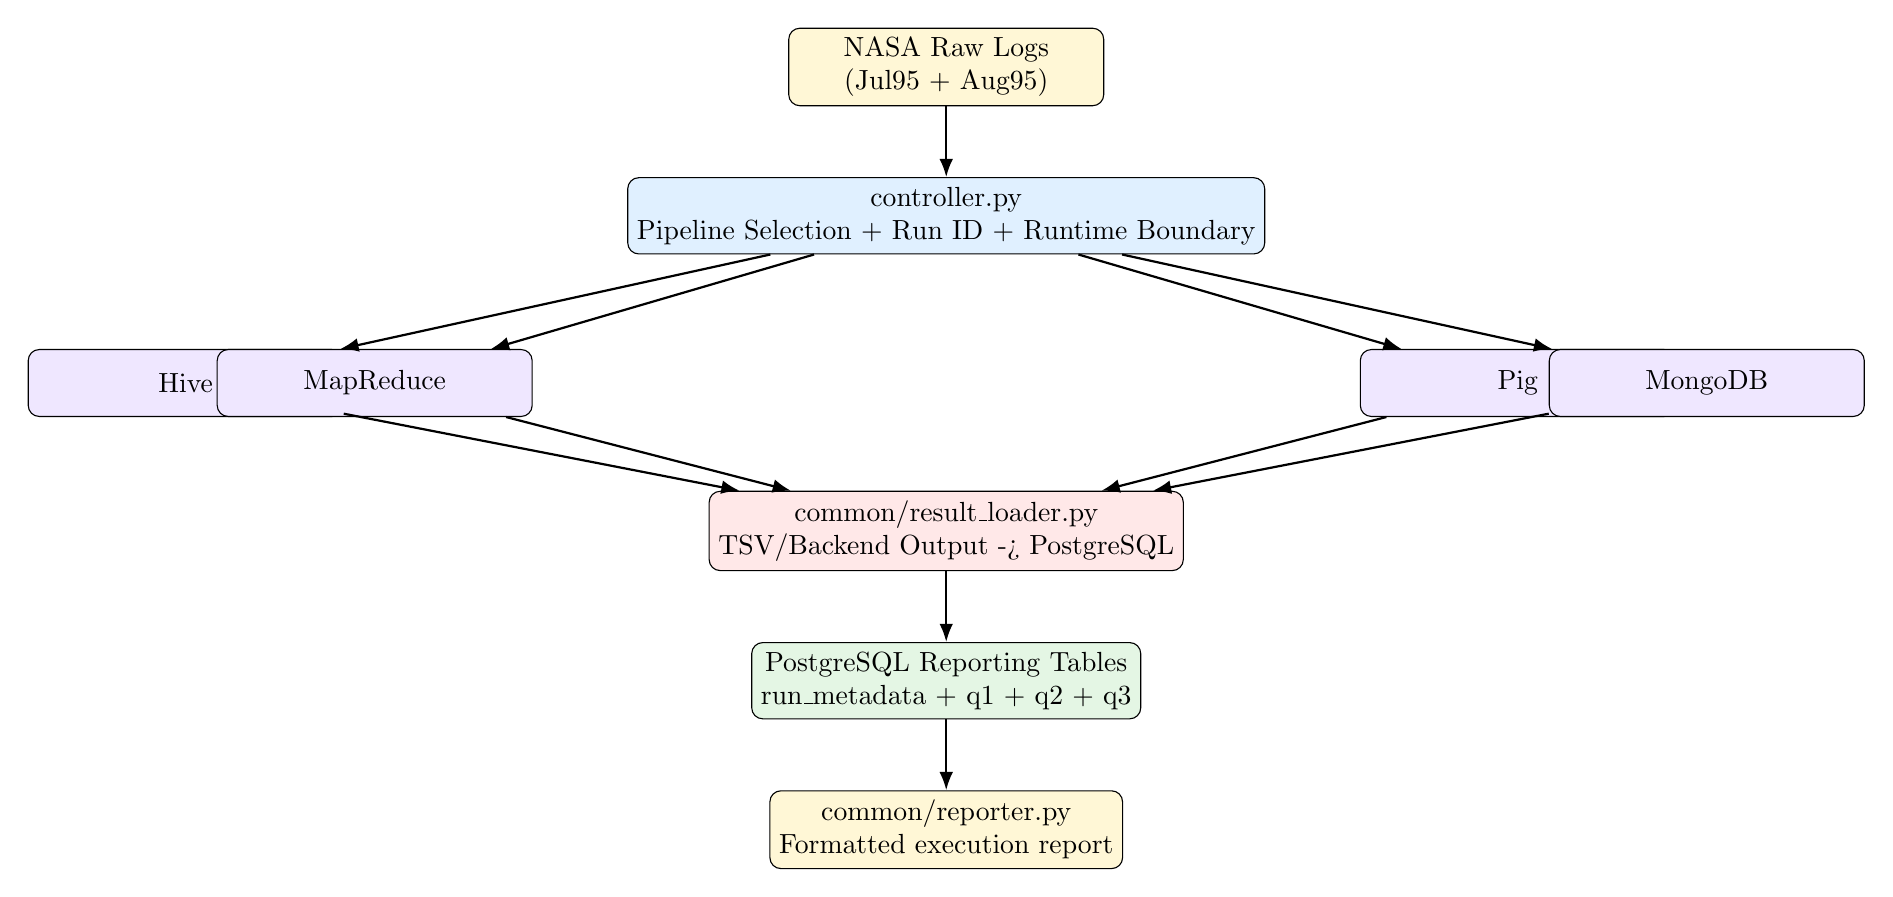
\begin{tikzpicture}[
    node distance=0.9cm,
    box/.style={rectangle, rounded corners, draw, align=center, minimum width=4.0cm, minimum height=0.85cm},
    arrow/.style={-Latex, thick}
]
\node[box, fill=flowyellow] (input) {NASA Raw Logs\\ (Jul95 + Aug95)};
\node[box, fill=flowblue, below=of input] (controller) {controller.py\\Pipeline Selection + Run ID + Runtime Boundary};
\node[box, fill=flowpurple, below left=1.2cm and 3.6cm of controller] (hive) {Hive};
\node[box, fill=flowpurple, below left=1.2cm and 1.2cm of controller] (mr) {MapReduce};
\node[box, fill=flowpurple, below right=1.2cm and 1.2cm of controller] (pig) {Pig};
\node[box, fill=flowpurple, below right=1.2cm and 3.6cm of controller] (mongo) {MongoDB};
\node[box, fill=flowred, below=3.0cm of controller] (loader) {common/result\_loader.py\\TSV/Backend Output -> PostgreSQL};
\node[box, fill=flowgreen, below=of loader] (db) {PostgreSQL Reporting Tables\\run\_metadata + q1 + q2 + q3};
\node[box, fill=flowyellow, below=of db] (reporter) {common/reporter.py\\Formatted execution report};

\draw[arrow] (input) -- (controller);
\draw[arrow] (controller) -- (hive);
\draw[arrow] (controller) -- (mr);
\draw[arrow] (controller) -- (pig);
\draw[arrow] (controller) -- (mongo);
\draw[arrow] (hive) -- (loader);
\draw[arrow] (mr) -- (loader);
\draw[arrow] (pig) -- (loader);
\draw[arrow] (mongo) -- (loader);
\draw[arrow] (loader) -- (db);
\draw[arrow] (db) -- (reporter);
\end{tikzpicture}
}
\caption{Unified architecture for the multi-pipeline ETL framework}
\end{figure}

\subsection{Holistic Multi-Pipeline Flow Diagram}
\begin{figure}[H]
\centering
\resizebox{0.95\textwidth}{!}{
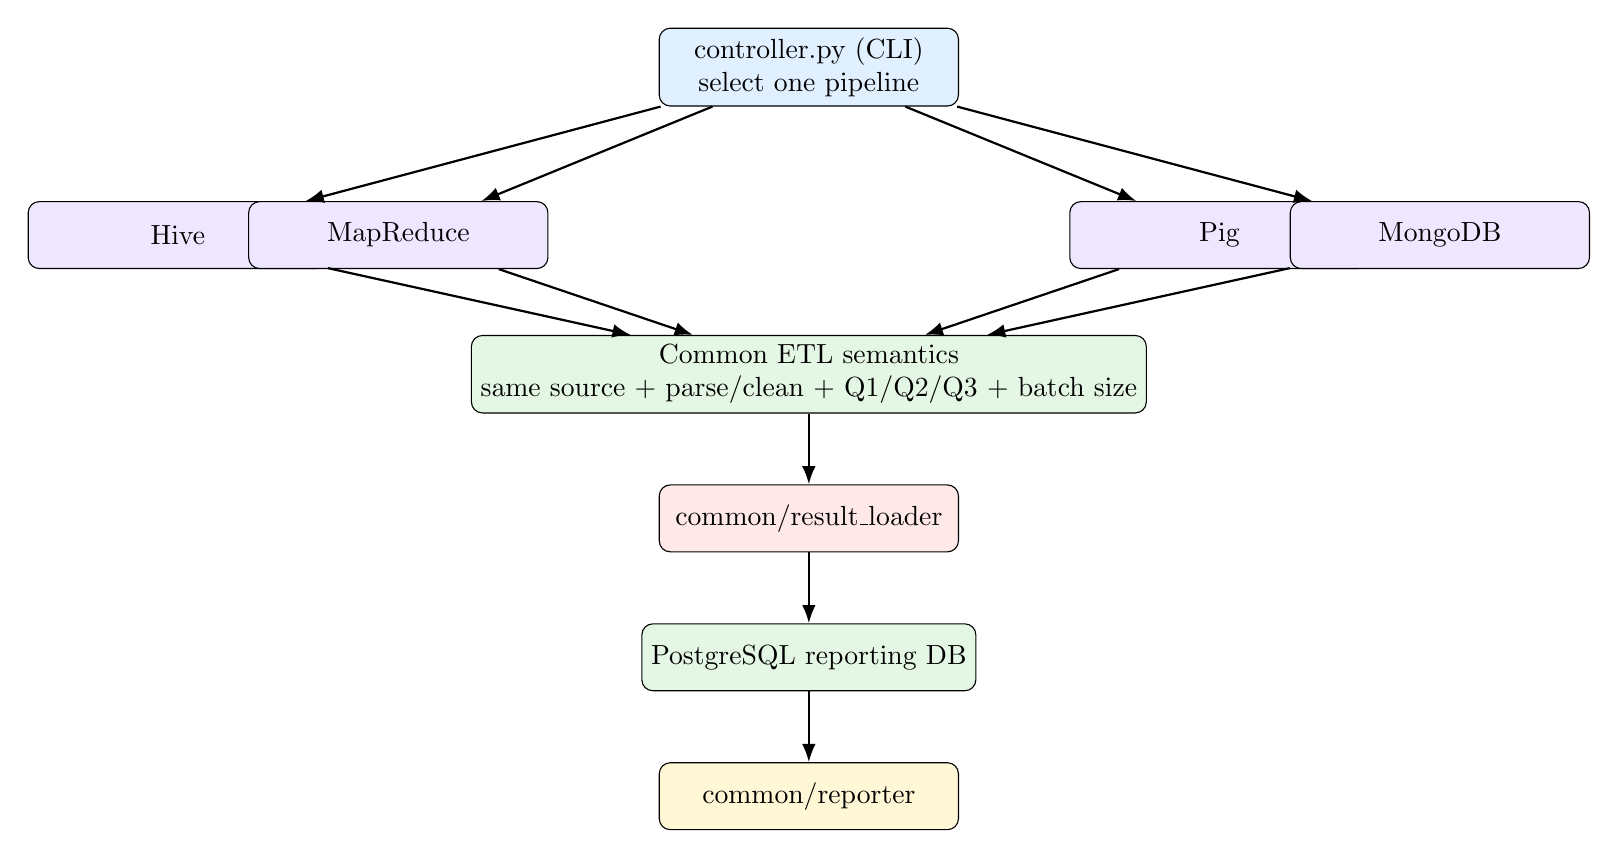
\begin{tikzpicture}[
    node distance=0.9cm,
    box/.style={rectangle, rounded corners, draw, align=center, minimum width=3.8cm, minimum height=0.85cm},
    arrow/.style={-Latex, thick}
]
\node[box, fill=flowblue] (cli) {controller.py (CLI)\\select one pipeline};
\node[box, fill=flowpurple, below left=1.2cm and 4.2cm of cli] (hive) {Hive};
\node[box, fill=flowpurple, below left=1.2cm and 1.4cm of cli] (mr) {MapReduce};
\node[box, fill=flowpurple, below right=1.2cm and 1.4cm of cli] (pig) {Pig};
\node[box, fill=flowpurple, below right=1.2cm and 4.2cm of cli] (mongo) {MongoDB};
\node[box, fill=flowgreen, below=2.9cm of cli] (semantics) {Common ETL semantics\\same source + parse/clean + Q1/Q2/Q3 + batch size};
\node[box, fill=flowred, below=of semantics] (loader) {common/result\_loader};
\node[box, fill=flowgreen, below=of loader] (db) {PostgreSQL reporting DB};
\node[box, fill=flowyellow, below=of db] (report) {common/reporter};

\draw[arrow] (cli) -- (hive);
\draw[arrow] (cli) -- (mr);
\draw[arrow] (cli) -- (pig);
\draw[arrow] (cli) -- (mongo);
\draw[arrow] (hive) -- (semantics);
\draw[arrow] (mr) -- (semantics);
\draw[arrow] (pig) -- (semantics);
\draw[arrow] (mongo) -- (semantics);
\draw[arrow] (semantics) -- (loader);
\draw[arrow] (loader) -- (db);
\draw[arrow] (db) -- (report);
\end{tikzpicture}
}
\caption{Holistic flow for interchangeable pipeline execution}
\end{figure}

%% ---------------------------------------------------------------
\section{Parsing Strategy}
%% ---------------------------------------------------------------
A single canonical parsing specification is enforced across all four pipelines to guarantee equivalence. The NASA traces follow an NCSA-style common web server log format with CLF-like core fields, as described in the assignment.

\subsection{Log Format}
Each line is structured as:
\begin{lstlisting}[language=bash]
host - - [DD/Mon/YYYY:HH:MM:SS -TZOFF] "METHOD /path HTTP/ver" status bytes
\end{lstlisting}
\textbf{Example:}
\begin{lstlisting}[language=bash]
199.72.81.55 - - [01/Jul/1995:00:00:01 -0400] "GET /history/apollo/ HTTP/1.0" 200 6245
\end{lstlisting}

\subsection{Canonical Regular Expression}
The following regex is the single source of truth. All four pipelines implement it exactly, with whitespace preserved explicitly:
\begin{lstlisting}
^(\S+)\s+\S+\s+\S+\s+\[(\d{2}/\w{3}/\d{4}):(\d{2}):\d{2}:\d{2}\s+[+-]\d{4}\]\s+"(\S+)\s+(\S+)\s+(\S+)"\s+(\d{3})\s+(\S+)$
\end{lstlisting}

Capture groups:
\begin{center}
\begin{tabular}{cll}
\toprule
\textbf{Group} & \textbf{Field} & \textbf{Notes} \\
\midrule
1 & \texttt{host}      & IP address or hostname \\
2 & \texttt{date\_str} & \texttt{DD/Mon/YYYY} -- converted to \texttt{YYYY-MM-DD} \\
3 & \texttt{hour}      & Integer 0--23 \\
4 & \texttt{http\_method}    & GET, POST, HEAD, \ldots \\
5 & \texttt{resource\_path}  & URL path \\
6 & \texttt{protocol\_version} & HTTP/1.0, HTTP/1.1 \\
7 & \texttt{status\_code}    & Integer \\
8 & \texttt{bytes}           & Integer; \texttt{-} $\rightarrow$ 0 \\
\bottomrule
\end{tabular}
\end{center}

\subsection{Cleaning Rules (identical across all pipelines)}
\begin{itemize}
    \item \textbf{Bytes field}: If the value is \texttt{-} or missing, it is replaced with \texttt{0}.
    \item \textbf{Date}: \texttt{DD/Mon/YYYY} is converted to ISO format \texttt{YYYY-MM-DD} using a fixed month-abbreviation map (Jan=01, \ldots, Dec=12). \texttt{log\_hour} is stored as an integer.
    \item \textbf{Malformed records}: If the regex match fails for any line, the line is \emph{not silently dropped}. The system increments a \texttt{malformed\_count} counter and reports the total at the end of the run. Malformed records are excluded from aggregations only.
\end{itemize}
All pipelines implement identical logical ETL steps (parse, transform, batch, aggregate) to ensure semantic equivalence.

%% ---------------------------------------------------------------
\section{ETL Workflow}
%% ---------------------------------------------------------------
The following five-step workflow is identical in logic across all pipelines. Only the implementation technology differs.

\begin{enumerate}
    \item \textbf{Extract}: Read raw NASA HTTP log lines from the configured source path. In the implemented Hive prototype, extraction is from \texttt{hdfs:///nasalogs/raw/} via an external Hive table.
    \item \textbf{Parse}: Apply the canonical regex to each line. Failed matches increment the malformed counter.
    \item \textbf{Transform}: Derive \texttt{log\_date} (YYYY-MM-DD) and \texttt{log\_hour} (integer) from the date string. Convert \texttt{bytes} (\texttt{-} $\rightarrow$ 0). Normalise \texttt{status\_code} to integer.
    \item \textbf{Batch \& Aggregate}: Assign \texttt{batch\_id} values (see Section~\ref{sec:batching}) and execute the three mandatory queries (Q1, Q2, Q3). Q2 is computed globally, while batch-aware metadata is preserved for reporting.
    \item \textbf{Load}: Write aggregated results and run metadata to PostgreSQL via \texttt{result\_loader.py}.
\end{enumerate}

Runtime measurement begins at the start of Step 1 and ends after Step 5 when aggregated rows are written to PostgreSQL. Report rendering time is excluded.

\subsection{Hive ETL File Execution Sequence (Implemented)}
\begin{verbatim}
Input source (HDFS): hdfs:///nasalogs/raw/
       |
       v
controller.py
  -> invokes pipelines/hive/run_hive.sh <batch_size> <run_id> <output_base>
       |
       v
run_hive.sh
  Step 1: executes 01_create_tables.hql
      Input : nasa_raw external table (HDFS raw lines)
      Output: nasa_parsed managed table with parsed fields + batch_id
  Step 2: executes 02_queries.hql
      Input : nasa_raw + nasa_parsed
      Output: local TSV folders under /tmp/etl_output/run_<id>/
          malformed/, q1/, q2/, q3/
       |
       v
controller.py
  -> invokes common/result_loader.py
       |
       v
result_loader.py
  Input : malformed/q1/q2/q3 TSV outputs
  Output: inserts run_metadata, q1_daily_traffic, q2_top_resources,
      q3_hourly_errors rows in PostgreSQL
       |
       v
controller.py updates final runtime_ms
       |
       v
controller.py -> common/reporter.py prints metadata + query outputs
\end{verbatim}

%% ---------------------------------------------------------------
\section{Batching Approach}
\label{sec:batching}
%% ---------------------------------------------------------------

\subsection{Parsing Strategy Diagram}
\begin{figure}[H]
\centering
\resizebox{0.92\textwidth}{!}{
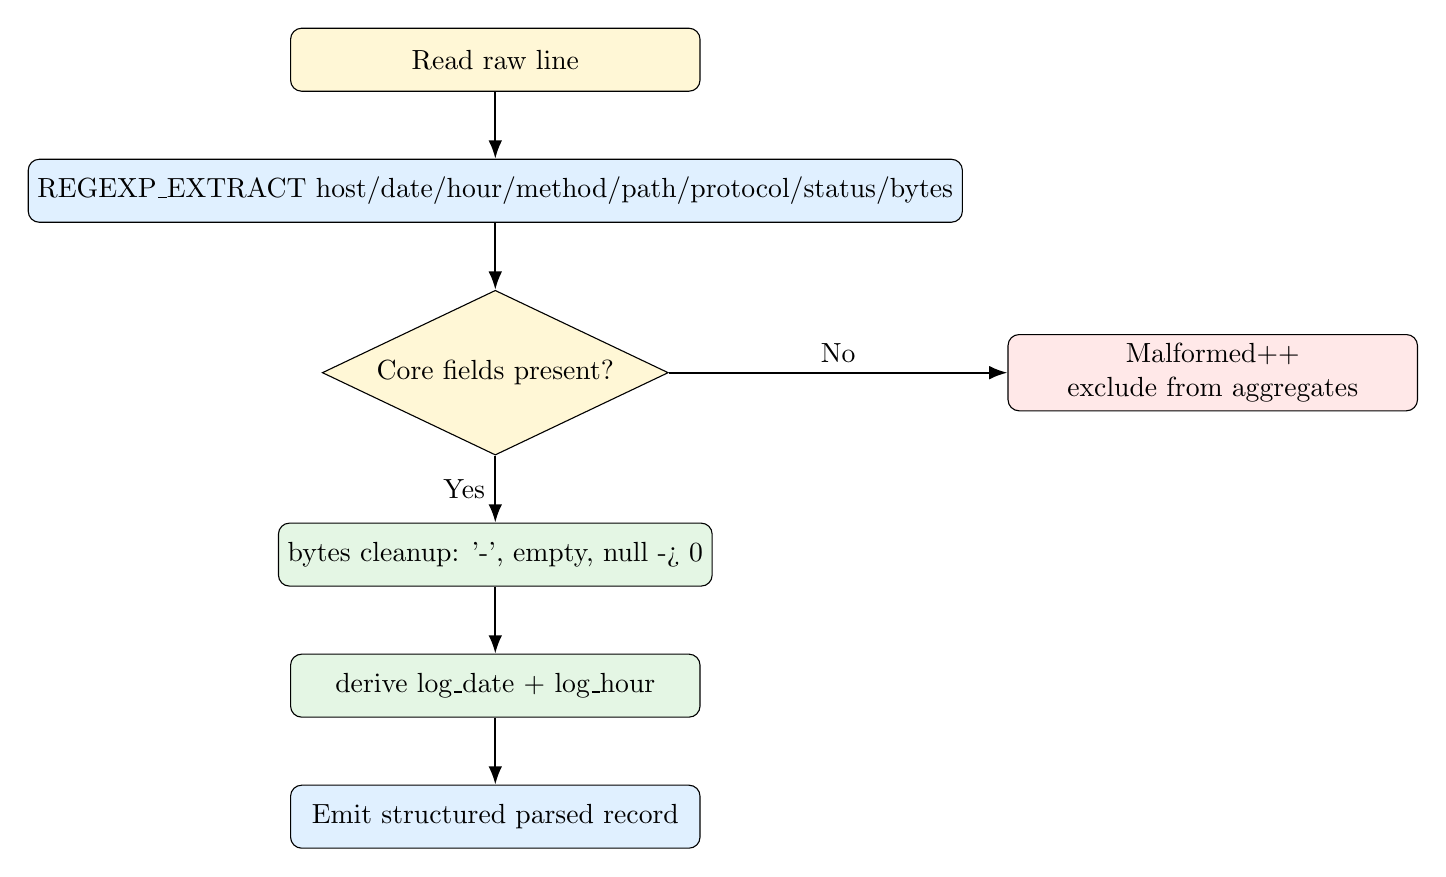
\begin{tikzpicture}[
    node distance=0.85cm,
    box/.style={rectangle, rounded corners, draw, align=center, minimum width=5.2cm, minimum height=0.8cm},
    decision/.style={diamond, draw, align=center, aspect=2.1, minimum width=3.2cm},
    arrow/.style={-Latex, thick}
]
\node[box, fill=flowyellow] (raw) {Read raw line};
\node[box, fill=flowblue, below=of raw] (extract) {REGEXP\_EXTRACT host/date/hour/method/path/protocol/status/bytes};
\node[decision, fill=flowyellow, below=of extract] (valid) {Core fields present?};
\node[box, fill=flowred, right=4.3cm of valid] (bad) {Malformed++\\exclude from aggregates};
\node[box, fill=flowgreen, below=of valid] (bytes) {bytes cleanup: '-', empty, null -> 0};
\node[box, fill=flowgreen, below=of bytes] (derive) {derive log\_date + log\_hour};
\node[box, fill=flowblue, below=of derive] (out) {Emit structured parsed record};

\draw[arrow] (raw) -- (extract);
\draw[arrow] (extract) -- (valid);
\draw[arrow] (valid) -- node[above]{No} (bad);
\draw[arrow] (valid) -- node[left]{Yes} (bytes);
\draw[arrow] (bytes) -- (derive);
\draw[arrow] (derive) -- (out);
\end{tikzpicture}
}
\caption{Parsing and cleaning flow used by the implemented Hive logic}
\end{figure}

\begin{itemize}
    \item \textbf{Batch size} ($N$): The number of input log records processed per batch. Passed as a CLI argument, identical across all pipelines in a given experiment.
    \item \textbf{Batch ID}: Monotonically increasing integer starting from 1. The final batch may contain fewer than $N$ records and is still counted as a valid batch.
    \item \textbf{Average batch size}: $\texttt{total\_records\_processed} \div \texttt{number\_of\_non\text{-}empty\_batches}$.
\end{itemize}

\subsection{Pipeline-Specific Batching}
\subsection{Batching Diagram (Implemented Hive Logic)}
\begin{figure}[H]
\centering
\resizebox{0.92\textwidth}{!}{
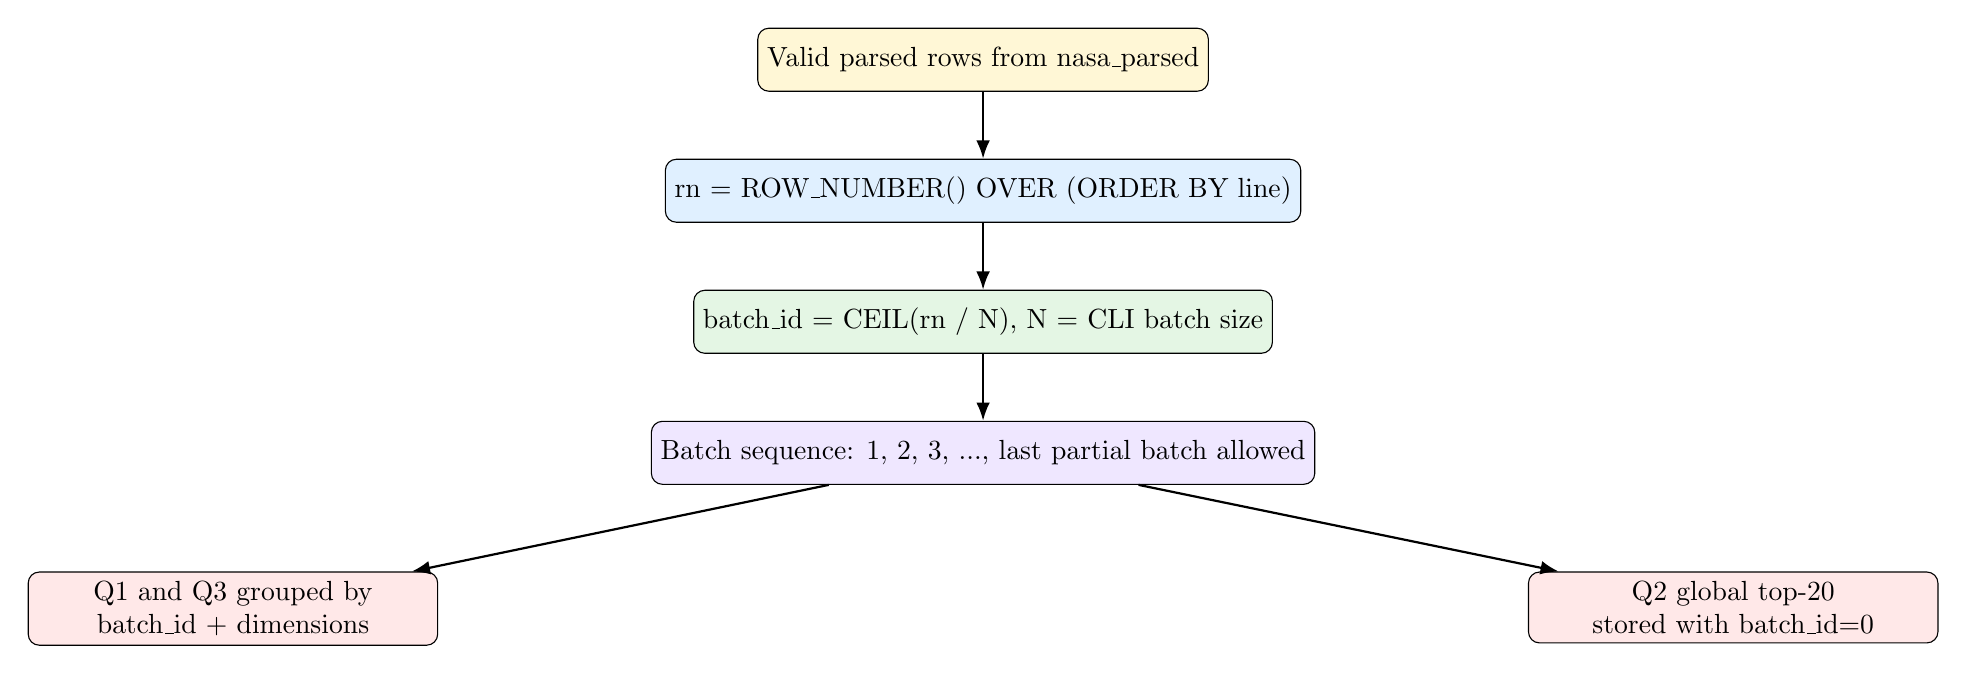
\begin{tikzpicture}[
    node distance=0.85cm,
    box/.style={rectangle, rounded corners, draw, align=center, minimum width=5.2cm, minimum height=0.8cm},
    arrow/.style={-Latex, thick}
]
\node[box, fill=flowyellow] (valid) {Valid parsed rows from nasa\_parsed};
\node[box, fill=flowblue, below=of valid] (rn) {rn = ROW\_NUMBER() OVER (ORDER BY line)};
\node[box, fill=flowgreen, below=of rn] (bid) {batch\_id = CEIL(rn / N), N = CLI batch size};
\node[box, fill=flowpurple, below=of bid] (seq) {Batch sequence: 1, 2, 3, ..., last partial batch allowed};
\node[box, fill=flowred, below left=1.1cm and 2.7cm of seq] (q1q3) {Q1 and Q3 grouped by\\batch\_id + dimensions};
\node[box, fill=flowred, below right=1.1cm and 2.7cm of seq] (q2) {Q2 global top-20\\stored with batch\_id=0};

\draw[arrow] (valid) -- (rn);
\draw[arrow] (rn) -- (bid);
\draw[arrow] (bid) -- (seq);
\draw[arrow] (seq) -- (q1q3);
\draw[arrow] (seq) -- (q2);
\end{tikzpicture}
}
\caption{Implemented batching logic and query batching behavior}
\end{figure}

\begin{center}
\begin{tabularx}{\textwidth}{lX}
\toprule
\textbf{Pipeline} & \textbf{Batching Mechanism} \\
\midrule
\textbf{Hive (Phase 1)} & Records are loaded into a staging table. A window function \texttt{CEIL(ROW\_NUMBER() OVER() / N)} assigns each row a \texttt{batch\_id}. Aggregations are then computed per \texttt{batch\_id}. \\
\addlinespace
\textbf{MapReduce (Phase 1)} & A custom \texttt{InputFormat} generates $N$-record splits from the \texttt{.gz} stream. Each split becomes one map task, corresponding to one \texttt{batch\_id}, injected via the Hadoop \texttt{Configuration} object. \\
\addlinespace
\textbf{Pig (Phase 2)} & A Python UDF tags each record with a \texttt{batch\_id} computed from its ordinal position within the input stream. \\
\addlinespace
\textbf{MongoDB (Phase 2)} & A Python loader streams the \texttt{.gz} file and calls \texttt{insertMany()} with slices of size $N$. Each \texttt{insertMany()} call corresponds to one \texttt{batch\_id}, stored as a field on every inserted document. \\
\bottomrule
\end{tabularx}
\end{center}

%% ---------------------------------------------------------------
\section{Mandatory Query Definitions}
%% ---------------------------------------------------------------
All three queries below are implemented identically in every pipeline. The SQL definitions serve as the canonical specification.

\subsection{Q1: Daily Traffic Summary}
\begin{lstlisting}[language=SQL]
SELECT batch_id, log_date, status_code,
       COUNT(*)   AS request_count,
       SUM(bytes) AS total_bytes
FROM parsed_logs
GROUP BY batch_id, log_date, status_code
ORDER BY batch_id, log_date, status_code;
\end{lstlisting}

\subsection{Q2: Top 20 Requested Resources}
\begin{lstlisting}[language=SQL]
SELECT resource_path,
       COUNT(*)             AS request_count,
       SUM(bytes)           AS total_bytes,
       COUNT(DISTINCT host) AS distinct_host_count
FROM parsed_logs
GROUP BY resource_path
ORDER BY request_count DESC
LIMIT 20;
\end{lstlisting}
Q2 is computed globally rather than per batch. In the reporting tables, it is stored with \texttt{batch\_id = 0} to distinguish it from batch-scoped aggregates.

\subsection{Q3: Hourly Error Analysis}
\begin{lstlisting}[language=SQL]
SELECT batch_id, log_date, log_hour,
  SUM(CASE WHEN status_code BETWEEN 400 AND 599 THEN 1 ELSE 0 END)
                                             AS error_request_count,
In the current implementation and report output, \texttt{error\_rate} is stored and displayed as a percentage in the range 0--100, rounded to 2 decimals.
  COUNT(*)                                   AS total_request_count,
  ROUND(SUM(CASE WHEN status_code BETWEEN 400 AND 599
                 THEN 1 ELSE 0 END) * 100.0 / COUNT(*), 2)
                                             AS error_rate,
  COUNT(DISTINCT CASE WHEN status_code BETWEEN 400 AND 599
                      THEN host END)         AS distinct_error_hosts
FROM parsed_logs
GROUP BY batch_id, log_date, log_hour
ORDER BY batch_id, log_date, log_hour;
\end{lstlisting}

%% ---------------------------------------------------------------
\section{Relational Reporting Database Schema}
%% ---------------------------------------------------------------
All pipeline results are stored in PostgreSQL using four tables: one for run metadata and one per query.

\subsection{Run Metadata}
\begin{lstlisting}[language=SQL]
CREATE TABLE run_metadata (
    run_id          SERIAL PRIMARY KEY,
    pipeline_name   VARCHAR(20) NOT NULL,  -- 'hive','mapreduce','pig','mongodb'
    run_timestamp   TIMESTAMP   NOT NULL,
    batch_size      INT         NOT NULL,
    total_records   BIGINT      NOT NULL,
    malformed_count BIGINT      NOT NULL DEFAULT 0,
    num_batches     INT         NOT NULL,
    avg_batch_size  NUMERIC(10,2) NOT NULL,
    runtime_ms      BIGINT      NOT NULL   -- read-start to final DB write
);
\end{lstlisting}

\subsection{Q1 Results Table}
\begin{lstlisting}[language=SQL]
CREATE TABLE q1_daily_traffic (
    id            SERIAL PRIMARY KEY,
    run_id        INT  REFERENCES run_metadata(run_id),
    pipeline_name VARCHAR(20) NOT NULL,
    batch_id      INT         NOT NULL,
    log_date      VARCHAR(10) NOT NULL,
    status_code   INT         NOT NULL,
    request_count BIGINT      NOT NULL,
    total_bytes   BIGINT      NOT NULL
);
\end{lstlisting}

\subsection{Q2 Results Table}
\begin{lstlisting}[language=SQL]
CREATE TABLE q2_top_resources (
    id                  SERIAL PRIMARY KEY,
    run_id              INT  REFERENCES run_metadata(run_id),
    pipeline_name       VARCHAR(20) NOT NULL,
    batch_id            INT         NOT NULL,
    resource_path       TEXT        NOT NULL,
    request_count       BIGINT      NOT NULL,
    total_bytes         BIGINT      NOT NULL,
    distinct_host_count BIGINT      NOT NULL
);
\end{lstlisting}

\subsection{Q3 Results Table}
\begin{lstlisting}[language=SQL]
CREATE TABLE q3_hourly_errors (
    id                   SERIAL PRIMARY KEY,
    run_id               INT  REFERENCES run_metadata(run_id),
    pipeline_name        VARCHAR(20) NOT NULL,
    batch_id             INT         NOT NULL,
    log_date             VARCHAR(10) NOT NULL,
    log_hour             SMALLINT    NOT NULL,
    error_request_count  BIGINT      NOT NULL,
    total_request_count  BIGINT      NOT NULL,
    error_rate           NUMERIC(6,2) NOT NULL,
    distinct_error_hosts BIGINT      NOT NULL
);
\end{lstlisting}

Execution time is recorded once in \texttt{run\_metadata.runtime\_ms} and associated with query rows through \texttt{run\_id}; this keeps the per-query tables focused on result payload while still preserving the time-of-execution metadata required by the assignment.

%% ---------------------------------------------------------------
\section{Plan for Ensuring Equivalence Across Pipelines}
%% ---------------------------------------------------------------
Equivalence across all four pipelines is guaranteed through the following mechanisms:

\begin{itemize}
    \item \textbf{Canonical Rules}: The canonical regex, cleaning rules, and query definitions are treated as fixed project-wide specifications and are reused across all backends.
    \item \textbf{Identical Input}: All pipelines use the same official NASA HTTP dataset source; no external cleaning, filtering, or schema conversion is allowed.
    \item \textbf{Identical Batch Size}: The batch size parameter $N$ is set via CLI and is identical for all pipelines in a given experiment.
    \item \textbf{Runtime Boundary}: All pipelines measure runtime identically -- from the moment input reading begins until the final aggregated result row is committed to PostgreSQL. Report rendering is excluded.
    \item \textbf{Cross-Pipeline Validation Plan}: During Phase 2, outputs from different \texttt{run\_id} values will be compared row-wise for Q1, Q2, and Q3 to verify semantic equivalence.
\end{itemize}

%% ---------------------------------------------------------------
\section{Output Formats: PostgreSQL and CSV Export}
%% ---------------------------------------------------------------

The reporting system supports two complementary output formats for persistence and accessibility:

\subsection{Primary Output: PostgreSQL Relational Database}
The main output target is PostgreSQL, where all results are normalized into four relational tables:
\begin{itemize}
    \item \texttt{run\_metadata}: pipeline execution metadata (batch size, runtime, record counts).
    \item \texttt{q1\_daily\_traffic}: daily traffic aggregates grouped by batch, date, and status code.
    \item \texttt{q2\_top\_resources}: global top-20 resources with distinct host counts.
    \item \texttt{q3\_hourly\_errors}: hourly error analysis grouped by batch, date, and hour.
\end{itemize}
All results include a \texttt{run\_id} foreign key for cross-table joins and run traceability.

\subsection{Secondary Output: CSV File Export}
In addition to PostgreSQL, all query results are automatically exported to CSV files organized by run ID. This provides:
\begin{itemize}
    \item \textbf{Accessibility}: CSV files can be opened in spreadsheet applications (Excel, LibreOffice) for immediate inspection.
    \item \textbf{Persistence}: Results are stored in a persistent file structure under \texttt{output/hive/run\_\{run\_id\}/} for long-term archive and reference.
    \item \textbf{Traceability}: Each run's outputs are isolated in a separate folder, making it easy to track and compare results across multiple runs.
\end{itemize}

\subsubsection{CSV Export Implementation}
After the PostgreSQL load completes, the controller invokes \texttt{common/export\_results.py}, which:
\begin{enumerate}
    \item Connects to PostgreSQL and retrieves all results for the current run.
    \item Exports metadata and all three query outputs as CSV files with headers.
    \item Stores files in \texttt{output/hive/run\_\{run\_id\}/} with standardized naming:
    \begin{itemize}
        \item \texttt{00\_run\_metadata.csv}
        \item \texttt{01\_q1\_daily\_traffic.csv}
        \item \texttt{02\_q2\_top\_resources.csv}
        \item \texttt{03\_q3\_hourly\_errors.csv}
    \end{itemize}
\end{enumerate}

This ensures that every run automatically generates a permanent, easily-viewable copy of its results without manual intervention.

%% ---------------------------------------------------------------
\section{Phase 1 Implementation Plan}
%% ---------------------------------------------------------------

\subsection{Pipeline 1: Apache Hive (Primary -- Phase 1)}
Hive is selected as the first pipeline because: (1) the three mandatory queries map directly to HiveQL; (2) Hive is already configured and verified on the development machine; (3) it supports a clean controller-driven execution flow; and (4) it minimises implementation time while fully satisfying Phase 1 prototype requirements.

\textbf{Implementation steps:}
\begin{enumerate}
    \item \texttt{01\_create\_tables.hql} -- creates external raw table and builds parsed/batched table using \texttt{REGEXP\_EXTRACT} and \texttt{ROW\_NUMBER()}.
    \item \texttt{02\_queries.hql} -- computes malformed count and executes Q1, Q2, and Q3 outputs.
    \item \texttt{run\_hive.sh} -- shell script to execute all HQL files in sequence.
    \item \texttt{result\_loader.py} -- reads Hive output files and inserts rows into PostgreSQL.
    \item \texttt{reporter.py} -- queries PostgreSQL and prints formatted output with metadata.
\end{enumerate}

\subsection{Pipeline 2: Apache MapReduce (Secondary -- Phase 1 if time permits)}
MapReduce is the second pipeline. It provides the strongest contrast (procedural vs.\ declarative) and demonstrates lower-level control over batching via a custom \texttt{InputFormat}.

\subsection{Pipelines 3 \& 4: Pig and MongoDB (Phase 2)}
Pig and MongoDB will be implemented after Phase 1. Both are fully designed in this document and will share the same \texttt{result\_loader.py} and \texttt{reporter.py} components with no changes required.

%% ---------------------------------------------------------------
\section{Project Directory Structure}
%% ---------------------------------------------------------------
\begin{verbatim}
End-Semester-Project/
|-- data/
|   |-- NASA_access_log_Jul95.gz
|   `-- NASA_access_log_Aug95.gz
|-- pipelines/
|   |-- hive/
|   |   |-- 01_create_tables.hql
|   |   |-- 02_queries.hql
|   |   `-- run_hive.sh
|   |-- mapreduce/
|   |   `-- src/
|   |-- pig/
|   `-- mongodb/
|-- common/
|   |-- result_loader.py
|   |-- reporter.py
|   |-- export_results.py
|-- schema/
|   `-- reporting_schema.sql
|-- controller.py
`-- output/
    `-- hive/
        |-- run_1/
        |   |-- 00_run_metadata.csv
        |   |-- 01_q1_daily_traffic.csv
        |   |-- 02_q2_top_resources.csv
        |   |-- 03_q3_hourly_errors.csv
        |-- run_2/
        `-- README.md
\end{verbatim}

\end{document}
